\chapter{Implementation}
This chapter includes the implementation of controllers and components. The chapter will be seperated into two section, a section for the inverted pendulum and another section for the rocket. An Arduino will be used as the platform to implement the hardware and software on.    


\subsection{MCU}\label{sec:MCU}
TBD

\todo{Sampling speed for both system, and argument that the arduino is fine with its 16 MHz clock speed.}

\section{Inverted Pendulum Implementation}
This section describes the implementation of the controller design cf. section \ref{sec:IPController}

\subsection{Implementing Sensors}
\todo{Consider the sampling speed of the sensors, when having the complete closed loop transfer function. - Mathias}


\subsubsection*{Potentiometer}\label{section:PotmeterImplementation}
The system consist of multiple sensors, as decribed cf. section \ref{sec:IPDesc}, where two of those is potentiometers. The potentiometers are linear Bourns 100 k$\Omega$. The potentiometers is tested cf. appendix \ref{appendix:PotMeterTest}. The appendix concluded with a first order approximation of both potentiometers. The approximation for Pot$_{arm}$ is:

\begin{equation}
\theta_a\ =\ 63,64 \cdot V_{{Pot}_{arm}} - 117,77
\end{equation}
\startexplain
	\explain{$\text{V}_{{Pot}_{arm}}$ is the output voltage of the  arms potentiometer}{V}
	\explain{$\theta_a$ is the angle of the arm}{$^\circ$}
\stopexplain

The approximation for Pot$_{stick}$ is:

\begin{equation}
\theta_s\ =\ 64,03 \cdot \text{VPot}_{stick} - 167,42
\end{equation}

\startexplain
	\explain{$\text{V}_{{Pot}_{arm}}$ is the output voltage of the stick potentiometer, but where zero degrees is when the stick has a zero degree deviation from the arm.}{V}
	\explain{$\theta_s$ is the angle of the stick}{$^\circ$}
\stopexplain

An example of implementing this is done trough a pseudo-code which converts the not limits to degree. Mapping can be used because of the linearity of the potentiometer.
\begin{lstlisting}
void loop() {
  // read the input on analog pin 0:
  int PotArm = analogRead(A0);
  int PotStick = analogRead(A1);
  if (PotArm >= 381 && PotArm <= 670)
  {
    int MappedPotArm1 = map(PotArm, 381, 670, 0, 90);
  }
  if (PotArm <= 380 && PotArm >= 89)
  {
    int MappedPotArm2 = map(PotArm, 380, 89, 0, -90);
  }
  if (PotStick >= 535 && PotStick <= 823)
  {
    int MappedPotStick1 = map(PotStick, 535, 823, 0, 90);
  }
  if (PotStick <= 534 && PotStick >= 248)
  {
    int MappedPotStick2 = map(PotStick, 534, 248, 0, -90);
  }
  delay(1);        // delay in between reads for stability
}
\end{lstlisting}    

In the code the approximations is not used, but can be implemented based on the execution time of the software.

The sampling time of the sensors can be is an important aspect when ensuring stability of the control system. The sensor sampling can not be to slow. Considering that the sensor is a potentiometer which does not have any active components then the only limit is the Arduino. Arduino specifies that calling a analogRead takes approximately 100 $\upmu$s which corresponds to a sampling frequency of 10 kHz. 

\subsubsection*{Tachometer}
The tachometer and its precision has been tested in appendix \ref{appendix:RPMTest}. The test concluded that the external optic A2108 tachometers precision is within the limit of what could implemented. The tachometer outputs a voltage which is linear with the number of revolutions per minute. It can be used in two modes, one where 1 V = 1000 rpm and one where 1 V = 10.000 rpm. This voltage can be used as an analogue input to the Arduino and then converted trough software. An example is seen in the following software sample: 

\begin{lstlisting}
void loop() {
  // read the input on analog pin 0:
  int TachoMeter = analogRead(A0);
  int VoltageTachoMeter = map(TachoMeter, 1, 1023, 0, 5) //Map the analog value back to a voltage so that the conversion is easier.
  int RadS = (VoltageTachoMeter * 1000) * 0.104719755 //Convert from RPM to rad/s
  Serial.println(RadS);
  delay(1);        // delay in between reads for stability
}
\end{lstlisting}  

Where the transfer function comes from datasheet and conversion from RPM to rad/s:
\begin{equation}
H_{tm}\ =\ \dfrac{\dfrac{1000\ \text{RPM}}{1\ \text{V}} \cdot 2 \cdot \pi}{60\ \text{s}}\ =\ 104,72\ \text{rad/s}
\end{equation}

\subsection{Implementing Motor Velocity Controller}
The following sections describes the implementation of the hardware motor controller with the Arduino. The motor driver in the setup is a Maxon Escon 50/5, which can be controlled with an Arduino trough PWM signals. 

The Maxon ESCON 50/5 is a PWM servo controller, that can be used to control DC and EC motors. The servo controller can be used in three different modes trough the Maxon ESCON studio. It can be configured in two modes for speed control with open and closed loops and feedback from sensors trough the board, and one mode for motor current control trough inputs from other modules. In setup the Escon controller is set to current control so that it is possible to input a PWM signal from the Arduino, which will correspond that 90\% duty cycle equals 10 A and 10\% equals -10 A. This means that 50\% will be 0 A. 

The main specifications of the ESCON is listed cf. table \ref{MaxonSpecifications}.

\begin{table}[htbp]
	\centering
	\begin{tabular}{llll}
	\hline
	Parameter & Value & Unit \\ \hline
	Supply voltage V$_{cc}$& 10-50 V & {[}V{]} \\
	Output voltage (max.) & 0,98$\cdot$ V$_{cc}$& {[}kg{]} \\
	Nominal output current & 5 & {[}A{]} \\
	Maximum output current (<20 s) & 15 & {[}A{]}\\
	Current control PWM frequency & 53,6 & {[}kHz{]}
	\end{tabular}
\caption{Maxon Escon 50/5 specifications.}
\label{MaxonSpecifications}
\end{table}
\todo{Ref to datasheet.}
The Escon Controller is powered with a Mean Well SP150-15 switching power supply, that converts 230 V to 15 V/10 A that can cover the supply area of the motor. The construction of the power supply is considered a black box, because limitation is set by the university when working with 230 V. The setup connections for using the Escon 50/5 with the inverted pendulum setup is seen cf. figure \ref{fig:MaxonSetup}.  
\begin{figure}[htbp]
\centering
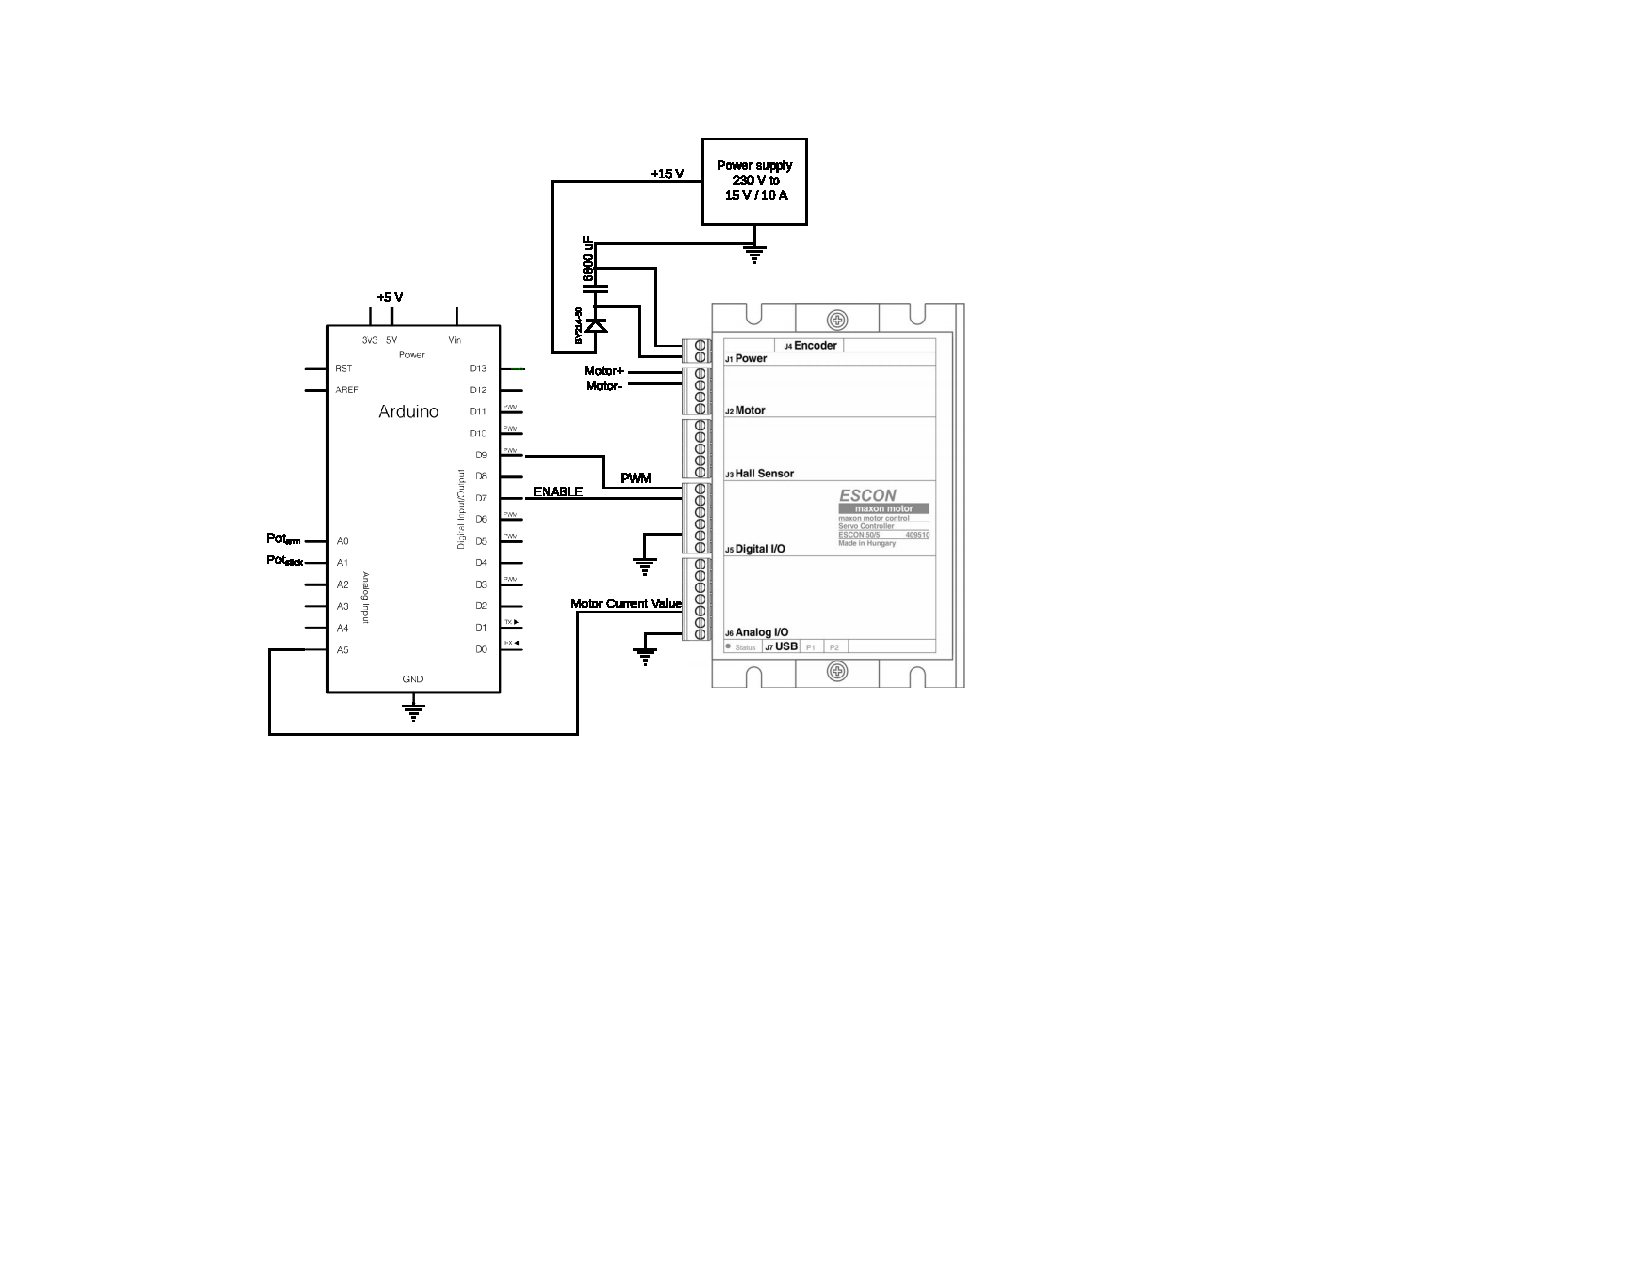
\includegraphics[width=1\textwidth]{figures/design/SetupMaxonDriver}
\caption{Setup for the Escon 50/5 motor controller.}
\label{fig:MaxonSetup}
\end{figure}
An example of implementing a proportional controller with the Escon 50/5 is found cf. \todo{CD/Software/??} where the setup of the Escon software is included.
\newpage



\section{Rocket Implementation}
TBD

\subsection{Implementing Inertial Measurement Unit}